\chapter{Implementation}

The algorithm is implemented as an extension to the Insight Segmentation and Registration Toolkit (ITK).  The ITK toolkit is a collection of image processing and statistical analysis algorithms that are relevant to biomedical imaging applications.  Additionally, the ITK toolkit is open-source software, which allows other researchers to learn directly how this system was implemented and possibly make improvements in the future.  Including the algorithm in the ITK toolkit provides a large existing research community access to the algorithm.  Additionally, a GUI module was created for the 3D Slicer medical visualization program that provides easy access to the algorithm via an intuitive visual interface.  Additionally,the ITK module can be used as a stand alone command line program suitable for non-interactive processing of large numbers of data sets.  Choosing to implement the algorithm as an extension of already established tools facilitate adoption of the algorithm in clinical studies.

The stochastic tractography algorithm is a monte carlo algorithm which samples the high dimensional parameter space of fiber tracts.  This parameter space is large because fiber tract are characterized by a sequence of segment orientations, each of which can be considered a separate parameter describing the fiber tract.  As such, it may take many samples to accurately approximate the posterior distribution of these parameters.  However, since these samples are IID, the samples can be generated in parallel.  Implementing the system in a multithreaded fashion enables parallel sampling of the tract distribution.

ITK  provides a framework for implementing some multithreaded algorithms.  The ITK multithreading framework assumes that the output region can be divided into disjoint sections with each thread working exclusively on their own section of the output image.  This design prevents threads from simultaneously writing to the same memory region, which may cause unexpected results.  However, since the stochastic tractography algorithm generates tracts that which may span the entire output image, dividing the output region into disjoint sections is not possible.  Additionally, we want to obtain statistics on these tracts so we need to output the generated tracts not just the resultant connectivity image.  Thus the existing ITK framework for implementing multithread filters is not very useful.  Fortunately ITK also provides basic multithreading functions which allows us to create a custom multithreaded design for the stochastic tractography system that is still within the ITK framework. 
\begin{figure} \label{fig:filterblock}
  \center
	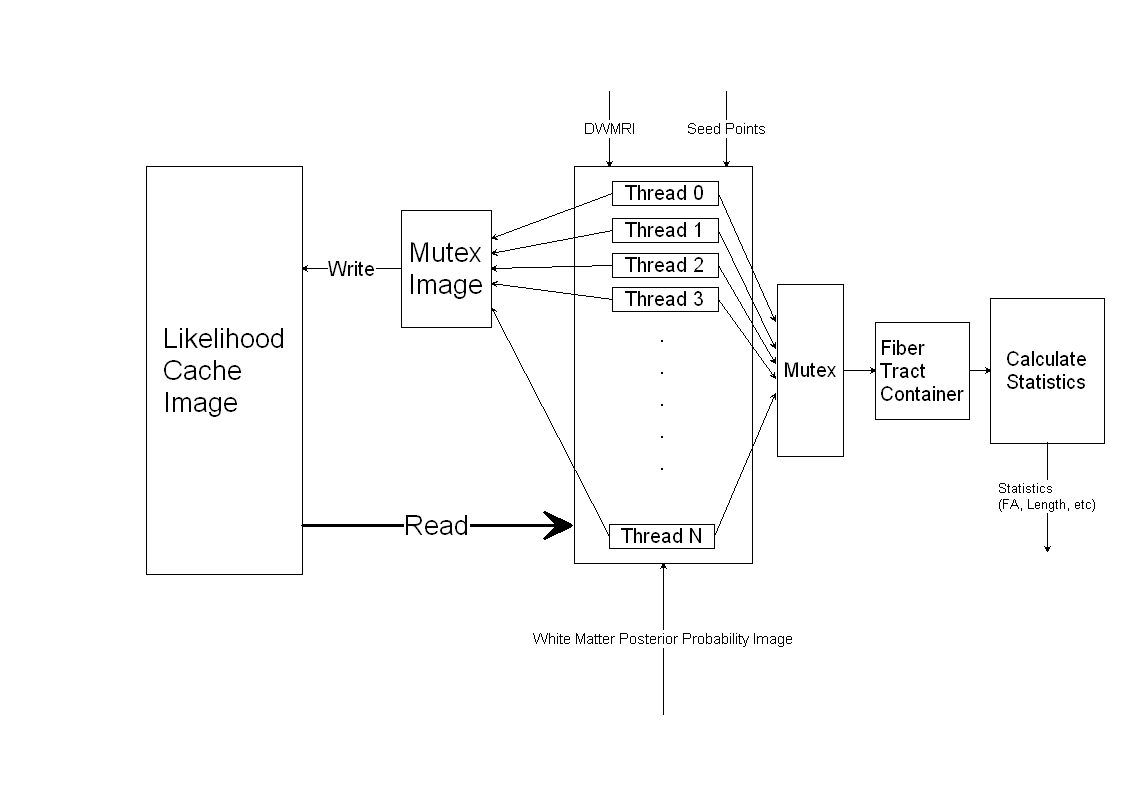
\includegraphics[width=\linewidth]{filterblock}
	\caption{A block diagram of the filter showing its shared likelihood cache and multithreaded architecture.}
\end{figure}
Each thread of stochastic tractography filter is an instance of the stochastic tractography algorithm. The block diagram in figure \ref{fig:filterblock} demonstrates graphically depicts the architecture of the ITK stochastic tractography filter.  Every thread allocates it own independent memory for the tract that it is currently generating.  Once the tract has terminated, the thread stores a memory pointer to the completed tract in a tract pointer container that is shared among all threads.  The tract pointer container is protected by a mutex, which serializes write operations so that only one thread can store its completed tract in the vector at a time.  Once the filter has generated enough samples, the tracts can be transferred to an output image to create a connectivity map.  Additionally other statistics can be computed on the tracts.  In essence, we divide the process into two sections, a multithreaded portion that samples the tracts and a single threaded portion which accumulates the tracts and calculates relevant statistics on them.

The most computationally expensive part of the algorithm is the calculation of the likelihood distribution.  The algorithm must compute probabilities for 2562 possible fiber orientations in a voxel.  Fortunately, this likelihood distribution is a deterministic function of the diffusion observations within that voxel.  The filter greatly improves its performance, at the cost of memory, by caching the generated likelihood distribution for later access.  Caching is very effective because in highly anisotropic regions of the brain, the sampled threads are expected to be dense causes many of the sampled tracts to visit the same voxels many times.

The cache is implemented as an image whose voxels are re-sizable arrays.  ITK's optimized pixel access capabilities enable quick access to the likelihood distribution associated with any voxel in the image.  On creation, every voxel in the likelihood cache image is initiated to a zero length array.  Whenever the algorithm encounters a voxel, it first checks to see if the likelihood cache contains this voxel by testing if associated array is zero length.  If the voxel has never been visited, the associated array is resized and the computation of the likelihood distribution associated with this voxel is stored inside the newly resized array.

Using a shared likelihood cache between multiple concurrent threads creates additional complexities.  Simultaneous writes to the cache will caused unexpected behavior.  Additionally there is the possibility of one thread will be reading incomplete cache information while another is trying to write it.  One possible solution is to ensure that only one thread can read or write to the likelihood cache at a time.  This is easily implemented by serializing access to the likelihood cache using a mutex.  A mutex serves as a lock on data.  A thread will wait to obtain a lock on the data before it proceeds to the next section of code.  Inside this section, which is called the critical section, the thread holds the lock ensuring exclusive access to the otherwise shared data.  All other threads must wait and idle while the thread which owns the lock finishes it operations.  Since threads must access the likelihood cache very often, this results in a situation where many threads are waiting for other threads to finish accessing the likelihood cache.  The serialized access to the likelihood cache creates a bottleneck, which in the worse case would result in performance that is only marginally better than a single threaded version of the filter.
\begin{figure} \label{fig:performance}
  \center
  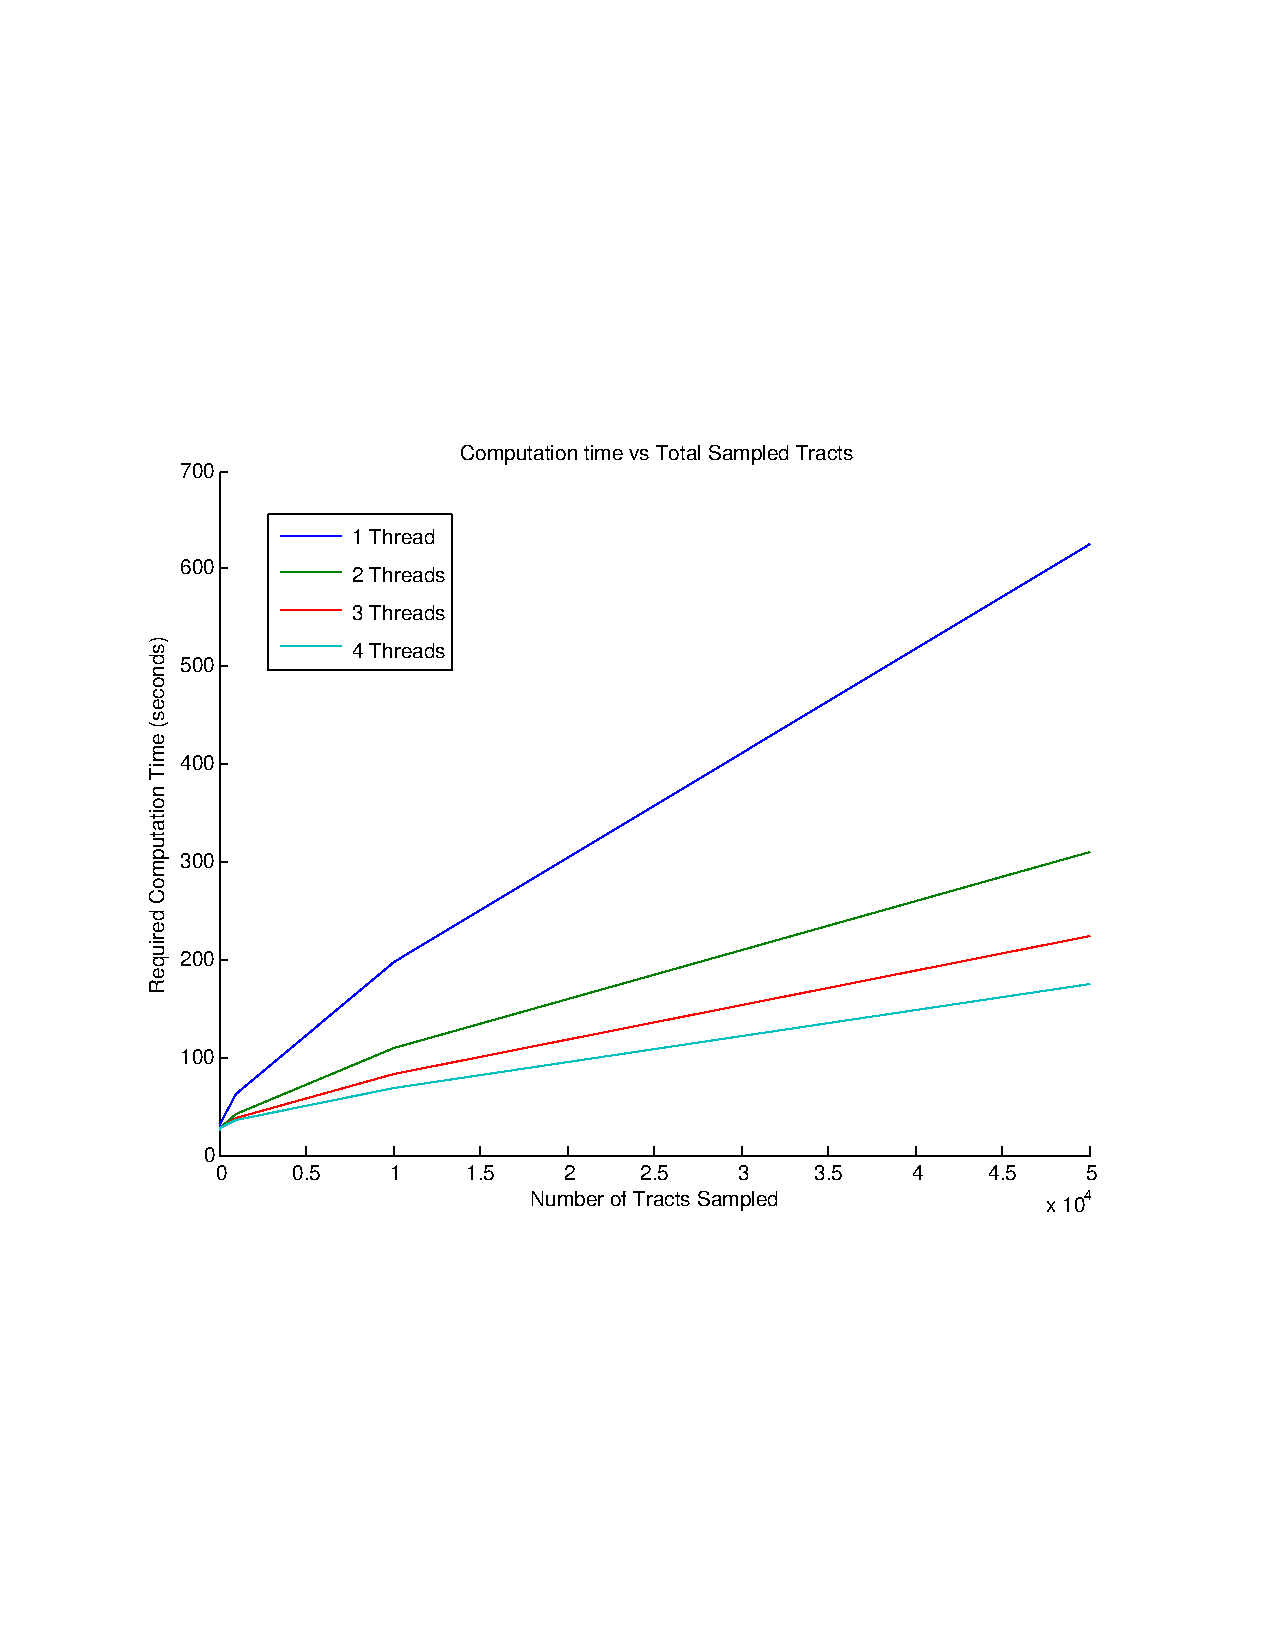
\includegraphics[trim = 20mm 70mm 20mm 70mm, clip, width=0.5\linewidth]
	  {timepertracts}
	\caption{A graph displaying the amount of time needed to sample a number of tracts.  Each line represents the algorithms performance using different numbers of threads.  This test was run on an 8 processor machine.}
\end{figure}

These access collisions to the likelihood cache can be reduced if we increase the granularity of the lock.  Instead of using one large lock for the entire likelihood cache image, we use a lock for each voxel.  The probability of two threads accessing the same voxel simultaneously is much less than the probability of two threads accessing any part of the likelihood cache.  These per voxel locks are conveniently constructed using an ITK image whose voxel data type is a mutex.  Similar to the likelihood cache, this collection of mutexes are indexed by coordinates which correspond to the coordinates of the voxels in the DWI input data.  Again, access to the mutex image is fast due to ITK's optimized access operators for data types indexed by coordinates.  The only cost to using this high resolution mutex image is the additional memory required to store these mutexes however this cost is small since a mutex is essential a boolean variable.  The mutex image allows different voxels in the likelihood cache image to be written to simultaneously, increasing the rate that the likelihood cache is filled.  The advantage of using a mutex image is most evident when tracking in highly isotropic regions,  where collisions are very unlikely to occur, since the sampled paths are very dispersed.  Even on uni-processor systems, using multiple threads may improve performance since the rate of encountering an unvisited voxel may be higher, thus filling the likelihood cache faster. Figure \ref{fig:performance} demonstrates the required computation time for a given number of tracts under different number of threads.

Additionally, to compute the WLS estimate for the tensor model parameters, we must first estimate the weights.  These weights are found by calculating a LS estimate of the true intensities of each voxel.  The $A$ matrix used in this LS estimation is a function solely of the magnetic gradient directions and associated b-values, which are the same for every voxel in the image.  Since the same $A$ matrix is used for each voxel in the LS calculation, a common optimization is to orthogonalize the $A$ matrix by computing its QR decomposition.  While this operation is computationally expensive but is only performed once for the entire DWI image.  The orthogonalized $A$ matrix reduces the cost of computing the weights for every voxel.

	

\section{3D Slicer Module}
\section{3D Slicer Interface}
\begin{figure} \label{fig:slicermodule}
  \center
	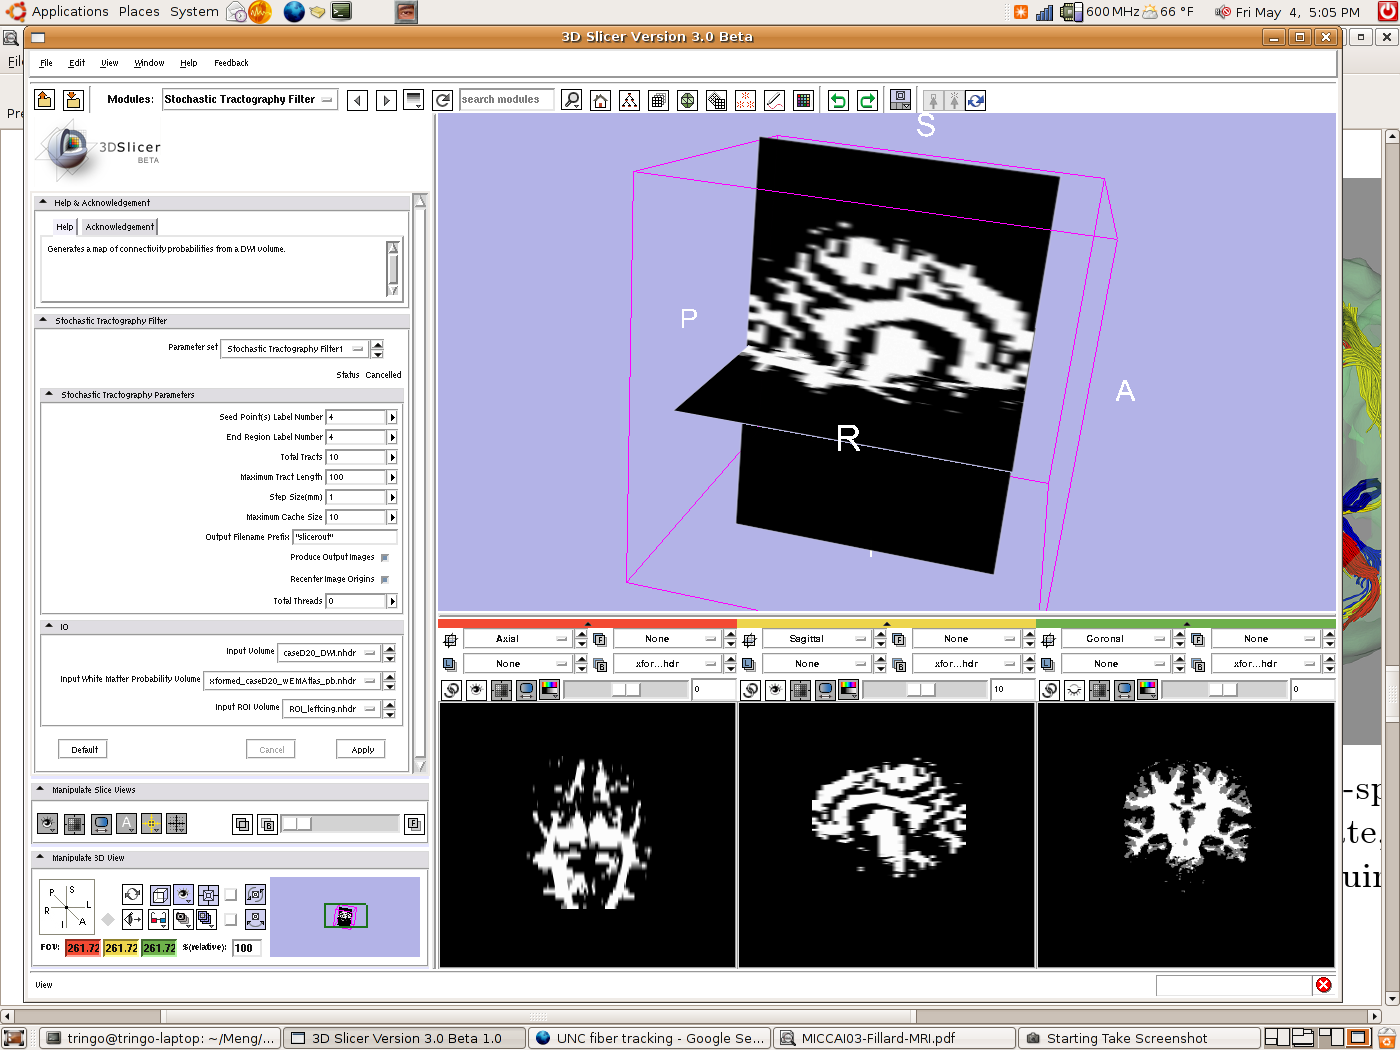
\includegraphics[width=0.5\linewidth]{slicermodule}
	\caption{This is a screen shot of the Stochastic Tractography GUI module with 3D Slicer.}
\end{figure}
%slicer3 module
%include figure
To encourage the algorithm's adoption in clinical studies an interactive GUI module for the 3D Slicer medical image visualization program was created which interfaces with the ITK stochastic tractography filter.  Figure \ref{fig:slicermodule} demonstrates the interface within the 3D Slicer environment.

The module was implemented using the command line module interface provided by the 3D Slicer environment.  This interface greatly eased the adaption of the command line interface into a graphical interface that could be included with 3D Slicer.  The command line interface and the graphical interfaces are both completely described using an XML file.  This XML file description is then parsed by a program provided by 3D Slicer which generates code that can be included with the command line interface to create what 3D Slicer refers to as a command line module.  Command line modules can be run independently of 3D Slicer but can also be incorporated in to the 3D Slicer graphical interface.  This enables the Stochastic Tractography system to function as an easy to use extension in the 3D Slicer program as well as a stand alone program suitable for processing a large numbers of data sets non-interactively.  Appendix B includes a detailed description of the options for the command line module.

%inputs
%outputs
%parameters

